\subsection{Señales ferroviarias}

    El sistema de señalamiento utiliza los semáforos ferroviarios (en adelante denominados señales) para indicarle al conductor del tren si tiene autoridad de tránsito en al próximo tramo de vías y a qué velocidad se le permite circular; esto, por medio del color de las señales, denominado aspecto. A diferencia de los semáforos vehiculares, en los que cada color es alternado por otro de la secuencia rojo-amarillo-verde en función del tiempo, las señales ferroviarios cambian su aspecto en función de los eventos de los tramos siguientes. En la Figura \ref{fig:signal_1} se presentan los posibles aspectos que pueden adoptar los semáforos utilizados en la gran mayoría de las líneas ferroviarias.

    \begin{figure}[!h]
        \centering
        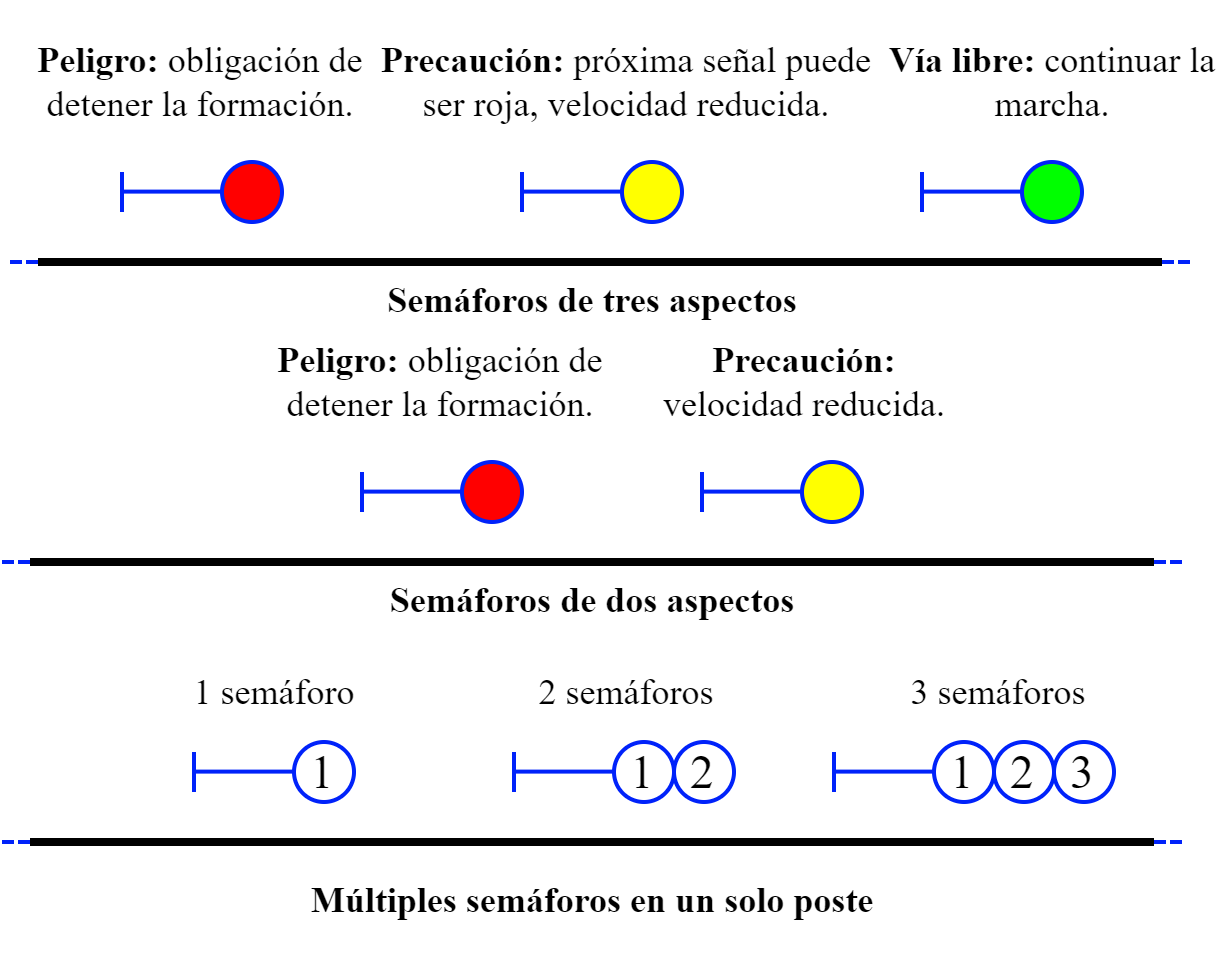
\includegraphics[width=1\textwidth]{Figuras/Semaforo3.png}
        \centering\caption{Aspectos de cada semáforo y múltiples señales en un semáforo.}
        \label{fig:signal_1}
    \end{figure}

    El tipo mas común de señal presenta tres aspectos, utilizado mayoritariamente en señales de circulación en vías principales. También existen las señales de maniobras, que se utilizan en cambios de vías donde, por su peligrosidad, solo se podrían permitir aspectos rojos (prohibido avanzar) y amarillos (precaución). Algunas líneas, como la Línea Roca, utilizan señales de cuatro aspectos, que poseen un doble amarillo antes del amarillo simple, para permitir así tramos de vías más cortos de forma segura.

    Varios señales pueden compartir físicamente un mismo poste, constituyendo un semáforo, como se visualiza en la Figura \ref{fig:signal_1}. De ahora en adelante, siempre que hablemos de un semáforo nos referimos al objeto físico o a un conjunto de señales que comparten un poste, mientras que hablaremos de señal como concepto abstracto o para referirnos a un solo semáforo del poste.
    
    A la hora de leer las señales de los semáforos de la Figura \ref{fig:signal_1}, consideramos al primer semáforo como el correspondiente a la rama principal de la red y a continuación todas la ramificaciones de derecha a izquierda, en el sentido de circulación de la formación. Esto permite simplificar el diagrama de señalamiento, concentrando varias señales que comparten una misma posición en un solo símbolo. Físicamente, las señales que comparten posiciones también comparten un poste o semáforo.

    En la Figura \ref{fig:signal_2} se ilustra la correspondencia de cada señal en el poste indicado como S01. Los colores del diagrama son meramente para indicar la correspondencia y no representan ningún aspecto. La señal S01 azul permite la circulación por la vía principal hasta la señal S02. La señal S01 verde permite la circulación por la primer ramificación, hasta la señal S03. Finalmente, la señal S01 roja permite la circulación por la vía secundaria mas a la izquierda de la formación, hasta la señal S04.

    \begin{figure}[!h]
        \centering
        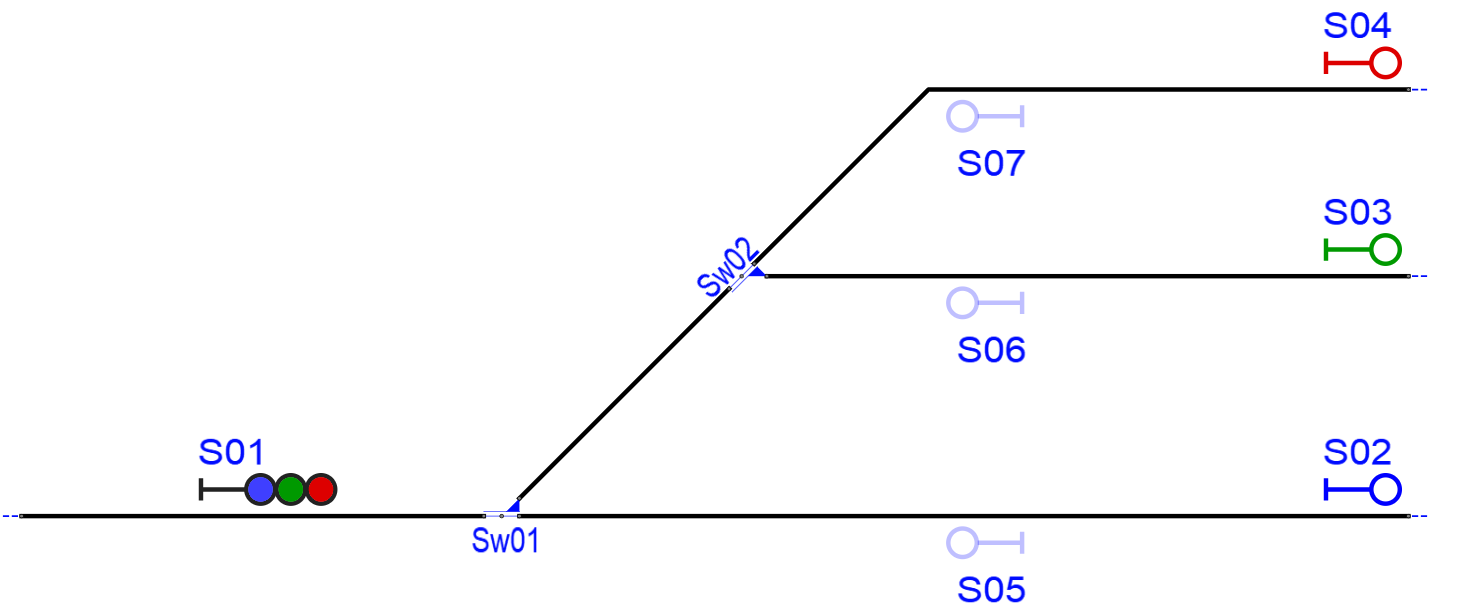
\includegraphics[width=1\textwidth]{Figuras/semaforos.PNG}
        \centering\caption{Ejemplo de asignación de señalización ramificada.}
        \label{fig:signal_2}
    \end{figure}

    Los semáforos siempre deben situarse a la izquierda del sentido de circulación. Por ejemplo, los semáforos S01, S02, S03 y S04 de la Figura \ref{fig:signal_2} son señales para un tren circulando de izquierda a derecha. Por otro lado, los semáforos S05, S06 y S07 son señales para un tren circulando de derecha a izquierda.